% \documentclass[preprint]{kcc}
\documentclass{kcc}


%%%%%%%%%%%%%%%%%%%%%%%%%%%%%%%%%%%%%%%%%%%%%%%
% include additional packages you need to use
%%%%%%%%%%%%%%%%%%%%%%%%%%%%%%%%%%%%%%%%%%%%%%%
% graphic, float package
\usepackage{graphicx}		% for setting images
\usepackage{float}			% for float objects
\usepackage{subfloat}		
\usepackage{subfigure}		% for adding several figures in a figure environment
\usepackage{lscape}			% for landscape type images or tables


\usepackage{enumitem}

% for compact section title spacing
% \usepackage[compact]{titlesec}


% mathmetical presentation
\usepackage{gensymb}
\usepackage{amsmath}
\usepackage{amssymb}
\usepackage{amsthm}
\usepackage{exscale}
\usepackage{textcomp}		% extra symbols


% for circled number
\newcommand{\cl}[1]{\textcircled{\scriptsize #1}}


% package for using algorithmic presentation
\usepackage{algorithmic}
\usepackage{algorithm}
% customize algorithmic environment
\renewcommand{\algorithmicrequire}{\makebox[40px]{\hfill\textbf{Input :}}}
\renewcommand{\algorithmicensure}{\makebox[40px]{\hfill\textbf{Output :}}}

% array and table presentation
\usepackage{array}
\usepackage{tabulary}
\usepackage{multirow}
\usepackage[table]{xcolor}
\usepackage{ctable}
\usepackage{booktabs}		% for typesetting tables at the level of publication		
							% do not use vertical rule
							
							\usepackage{times}
\usepackage{CJKutf8}
\usepackage{mathrsfs}
\usepackage{verbatim}
\usepackage{amsfonts}
\usepackage{xspace}
\usepackage{xcolor}
\usepackage{url}
\usepackage{balance}
\usepackage{booktabs}
\usepackage{multirow}
\usepackage{rotating}
\usepackage{fancyvrb}
\usepackage{lastpage}
\usepackage{alltt}
\usepackage{etoolbox}
\usepackage{cleveref} % After hyperref, listings
\usepackage{fancyhdr}
\usepackage{listings}

\usepackage{caption}


% set title, author, abstract
\title{매니코어 환경에서 PARSEC 벤치마크 ROI 확장성 분석}
\author{
}
\engtitle{An Analysis of ROI Scalability on PARSEC \\Benchmark for Many-core
System} \engauthor{
}
\abstract{
본 논문은 최신 리눅스 커널인 4.11-rc8을 대상으로 100코어 이상의 매니코어 환경에서 
멀티 스레드 기반 워크로드에 대해서 대한 문제점을 제시하였다.
이를 위해 공유 메모리를 사용하는 환경에서 리눅스의 확장성에 대한 문제점을 분석하였다.
문제점을 분석하기 위해 멀티 스레드 기반 벤치마크인 PARSEC 벤치마크를 사용하였으며, 워크로드의 
병력화 부분인 ROI(Regine of Interest)의 부분만 추출 후 측정하여 확장성을 분석하였다.
분석 결과 대부분 워크로드가 확장성에 대해서 문제점을 가지며, 코어 수가 증가 할 수록 
커널에서 많은 시간을 소모 하였다.
}

\begin{document}

\maketitle

\section{서 론}
코어 수가 증가함에 따라 서버 환경이 멀티코어에서 매니코어로 증가하고 있다. 
이러한 매니코어 환경에 대해서 리눅스 커널의 확장성은 굉장히 중요하다. 
그동안 리눅스의 확장성을 분석하기 위한 많은 연구들이 진행되어 왔다~\cite{Etri}. 

우리의 이전 연구는 멀티 프로세스 워크로드를 대상으로 리눅스 커널에 대한 확장성에 
대해서 문제점을 제시하였고, 문제를 해결 하였다~\cite{kesl1}~\cite{kesl2}. 
하지만 실제 공유 메모리 환경에서는 멀티 프로세스 기반의 워크로드보다는 멀티 스레드 기반의 
워크로드가 더 많은 상황이다.

그동안 멀티 스레드 기반의 확장성 문제도 해결하고자 시도가 있었으며, 
그 중 리눅스 커널의 address space 문제인 mmap/munmap 과 페이지 폴트간의 경쟁 
때문에 발생하는 문제를 해결하는 연구들이 있었다~\cite{AustinTClements2012RCUBalancedTrees}. 
하지만 이런한 연구들은 복잡성과 안정성 때문에 
여전히 모두 최신 리눅스 커널에 반영되지 못하고 있다.

리눅스 커널은 확장성을 위해 많은 패치들이 적용되고 있다. 
따라서 최신 리눅스 커널의 확장성을 분석하는 것도 중요하다. 
본 연구는 이처럼 최신 리눅스 커널을 대상으로 
공유 메모리 기반의 매니코어 시스템에서 멀티 스레드를 
대상으로 확장성을 분석하였다.

분석은 멀티 스레드 기반 워크로드로 이루어진 PARSEC 벤치마크~\cite{parsecbench}를 이용하였으며, 각 워크로드 중
실제 병렬화가 수행되는 구간인 ROI(Regine of Interest)의 확장성을 분석하였다. 
본 연구는 향후 100코어 이상의 공유 메모리 기반의 매니코어 확장성 연구에 대해서 
반드시 필요한 사전 연구이다.

-----------------------------------------------------------------------------
* 본 연구는 xx




\section{관련 연구}

멀티 스레드기반의 워크로드를 대상으로 리눅스 커널의 확장성 분석에 대한 연구는 리눅스의 
address space에서 사용되는 동기화 기법인 mmap\_sem 때문에 발생하는 문제를 RCU기반의 
address space를 개발한 BonsaiVM~\cite{AustinTClements2012RCUBalancedTrees}이 있다.
다음으로 BonsaiVM의 문제점인 write 간의 병목을 해결하기 위해 address space가 중복되지 
않도록 자료구조를 구성하는 연구인 RadixVM~\cite{Clements2013RadixVM}이 있다.

\section{실험 환경}

실험 환경은 그림 ~\ref{fig:parsec}와 같으며, 120코어 인텔 xeon기반의 8소켓 머신이다. 
\begin{figure}[h]
  \begin{center}
     \includegraphics[width=0.3\textwidth]{fig/xeon}
  \end{center}
  \caption{매니코어 실험 환경 .}
  \label{fig:xeon}
\end{figure}

\begin{figure*}[tb!]
    \centering
    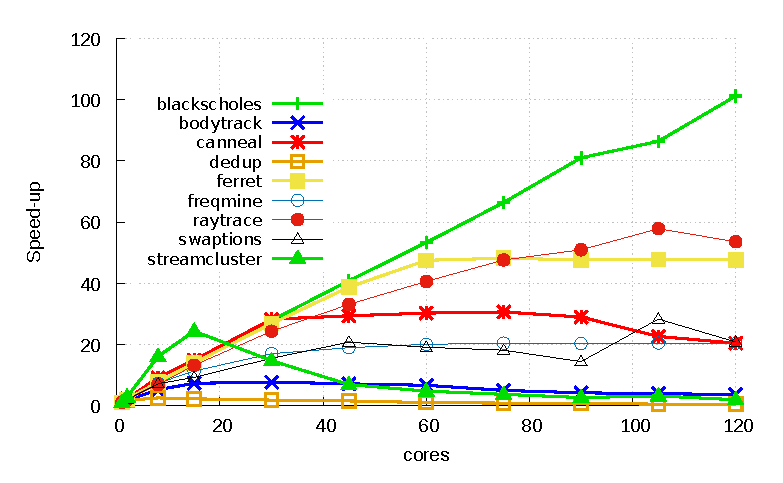
\includegraphics[width=4.8in]{graph/PARSEC.eps}
    \caption{벤치마크 실험 결과.}
    \label{fig:parsec}
\end{figure*}

측정 환경은 표 ~\ref{tab:config}와 같은 버전의 소프트웨어를 이용하였다. 
그리고 입력 데이터는 PARSEC 벤치마크에서 제공하는 native를 이용하였다.

\begin{table}[h!]
  \caption{소프트웨어 버전 및 입력 데이터.}
  \centering
  \small
  \begin{tabular}{l l l l l} \toprule
    운영체제 & 배포판 & PARSEC 버전 & 입력 데이터\\
    \midrule
    Linux 4.11-rc8 & Ubuntu 14.04 & PARSEC 3.0 & Native & \\
    \bottomrule
  \end{tabular}
  \label{tab:config}
\end{table}


\section{워크로드 설명}
본 연구에서는 PARSEC 벤치마크 중 9개의 벤치마크를 대상으로 측정을 하였다. 
각 워크로드의 설명과, 벤치마크에서 강조하고 있는 Data의 공유 정도 그리고
 락과 배리어등의 동기화 기법의 수에 대한 정보는  표~\ref{tab:workload}와 같다~\cite{parsecbench}.

\begin{table}[h!]
  \caption{워크로드 설명}
  \centering
  \scriptsize 
  \begin{tabular}{l l l l l} \toprule 
    워크로드명 &  & 데이터 공유 & 동기화 수 & 병렬화 모델\\
    \midrule
    blackscholes & 재정 분석 & 낮음 & 8 & data-parallel\\
    \midrule
    bodytrack & 컴퓨터 비젼 & 높음 & 2661 & data-parallel\\
    \midrule
    canneal & Engineering & 높음 & 34 & unstructured\\
    \midrule
    dedup & 엔터프라이즈 저장소 & 높음 & 160598 & pipeline\\
    \midrule
    ferret & 유사 검색 & 높음 & 345778 & pipeline\\
    \midrule
    freqmine & 데이터 마이닝 & 높음 & 990025 & data-parallel\\
    \midrule
    raytrace & 재정 분석 & 낮음 & 23 & data-parallel \\
    \midrule
    streamcluster & 데이터 마이닝 & 낮음 & 129918 & data-parallel\\
    \midrule
    swaptions & 재정 분석 & 낮음 & 23 & data-parallel \\
    \bottomrule
  \end{tabular}
  \label{tab:workload}
\end{table}

\section{워크로드 및 확장성 실험 결과}
 이번 장에선 본 연구는 두가지의 실험 결과를 바탕으로 결과를 도출해 내었다. 모든 실험은 15회 기준 평균 값으로 진행되었다.
첫번째로 각 프로그램마다 지정한 ROI가 프로그램의 확장성에 영향을 끼치는지를 확인하고 실험한 프로그램당 스레드별 실행시간을 기준으로 확장성을 확인해보았다.
\subsection{ROI (Region Of Interest)}
 먼저 ROI 부분이란 실제 병렬화되어서 실행되는 구간이다. 이 구간을 제외한 부분은 프로그램 실행시 필요한 초기화 부분이 대부분을 차지하고 있다. 표 ~\ref{tab:ROI_ratio}에서 확인할 수 있는 정적인 실행시간을 제외하고, ROI 부분만 확인 하였을때 모든 프로그램에서 최대 스레드 x0.7 수준의 성능향상이 있었다. 이로 비추어 볼때 실제로 우리가 측정하는 ROI시간들이 프로그램의 성능을 측정한다고 볼 수 있다.
\begin{table}
\caption{비 ROI 실행 시간} 
\label{tab:ROI_ratio}
\centering
\begin{tabular}{c|c|c}
\hline
워크로드 명 & 평균 실행시간 (s) & 전체 대비 비(\%) \\ \hline
blackscholes & 21.23 & 12.3 \\ \hline
bodytrack & 0.10 & 0.2 \\ \hline
canneal & 47.37 & 8.7 \\ \hline
dedup & 0.74 & 2.7\\ \hline
ferret & 0.18 & 0.1\\ \hline
freqmine & 0.08 & 0.1\\ \hline
raytrace & 59.52 & 25.9\\ \hline
streamcluster & 0.01 & 0.1\\ \hline
swaptions & 0.01 & 0.1\\ \hline
\end{tabular}
\end{table}
\subsection{실험 결과}
해당 실험결과는 native 입력 데이터셋을 기준으로 스레드 숫자를 늘려가며 기대하는 선형적인 확장성을 보여줄 수 있는지 확인한 결과이다. 가장 좋은 결과를 보여준 blackscholes 를 제외하고 A,B 그룹 2가지로 나누어서 결과를 유추할 수 있다.
\begin{itemize}
\item \textbf{blackscholes} :
해당 프로그램의 비 ROI 실행 시간은 대부분을 입력 값을 초기화하는 곳에 사용한다. 또한 표 ~\ref{tab:workload} 에서 확인 할 수 있듯이 동기화와 데이터 공유의 빈도가 매우 낮다. 이로 인해서 완벽한 선형은 아니지만 다른 8개의 벤치마크에 비해서 가장 높은 멀티스레딩 대비 확장성을 보여준다.
\item \textbf{A 그룹} (bodytrack,canneal,dedup,ferret,freqmine) : 해당 그룹에 속하는 프로그램들은 모두 동기화와 데이터 공유의 빈도가 매우 높다. 결과도 성능이 비교적 완만하게 증가하다가 오히려 10~20 스레드 사이에서부터 성능의 하락이 일어나고 있다. 따라서 측정된 프로그램들 중 가장 확장성이 낮은 그룹이라고 볼 수 있다.
\item \textbf{B 그룹} (streamcluster,raytrace,swaption) : 해당 그룹에 속하는 프로그램들은 동기화 빈도는 높지만 데이터공유의 정도가 낮은 그룹이다. 그림 ~\ref{fig:parsec} 에서 그룹 B 에 속해있는 프로그램들의 그래프를 살펴보면, 오히려 스레드 숫자가 50개 정도일 때 까지는 선형적인 확장성을 보이고 있다. 심지어 streamcluster 의 경우 스레드가 낮을때에 국한해서 blackscholes 의 확장성을 훨씬 웃돌고 있다. 하지만 모두 일정 스레드 이후에는 성능이 더이상 증가하고 있지 않다.
\end{itemize}

\begin{table}[]
\centering
\caption{결과그룹}
\label{tab:result_group}
\begin{tabular}{|c|c|}
\hline
\multicolumn{2}{|c|}{데이터 공유}                                                                                                                                         \\ \hline
높음                                                                                   & 낮음                                                                            \\ \hline
\begin{tabular}[c]{@{}c@{}}bodytrack,dedup,canneal\\ ferret,freqmine(A)\end{tabular} & \begin{tabular}[c]{@{}c@{}}streamcluster\\ raytrace,swaptions(B)\end{tabular} \\ \hline
\end{tabular}
\end{table}
\section{결론 및 향후 연구}

PARSEC의 ROI 부분만 측정하여 분석한 결과 PASEC의 대부분의 워크로드는 확장성에 문제를 
가지고 있다. 특히 표 ~\ref{tab:result_group}의 그룹 A와 B 를 비교해보았을때 데이터공유 문제가 스레드가 많아지면 많아질 수록 부각 되는 것을 확인할 수 있었다.  PARSEC은 공유 메모리 기반의 멀티 쓰레드를 이용한 워크로드로 구성되어 있는 벤치마크이다.
향후 연구로는 본 연구의 결과를 이용하여 리눅스의 매니코어 시스템에서 멀티 쓰레드의 
문제점을 분석할 예정이다.

\bibliographystyle{ieeetr}
\begin{thebibliography}{7}
\bibitem{Etri}
정진환, 김강호, 김진미, 정성인. 
\newblock Manycore 운영체제 동향. 
\newblock 전자통신 동향 분석 29권 5호, 2014. 
\bibitem{kesl1}
경주현, 임성수.
\newblock 매니코어 시스템을 위한 리눅스 가상 메모리 관리의 락 경합 분석. 
\newblock 한국정보과학회, 한국정보과학회 학술발표논문집 , 2015.6, 1571-1573, 2015
\bibitem{kesl2}
경주현, 윤성민, 임성수.
\newblock 매니코어 환경에서 로그 기반 동시적 업데이트 기법을 활용한 리눅스 커널 확장성 개선.
\newblock 한국정보과학회 학술발표논문집 , 2016.12, 512-513, 2016
\bibitem{AustinTClements2012RCUBalancedTrees}
Austin~T. Clements, M.~Frans Kaashoek, and Nickolai Zeldovich.
\newblock Scalable address spaces using {RCU} balanced trees.
\newblock In {\em Architectural Support for Programming Languages and Operating
  Systems (ASPLOS 2012)}, pages 199--210, London, UK, February 2012.
\bibitem{parsecbench}
Bienia, Christian and Kumar, Sanjeev and Singh, Jaswinder Pal and Li, Kai
\newblock The PARSEC benchmark suite: characterization and architectural
implications.
\newblock PACT '08 Proceedings of the 17th international
conference on Parallel architectures and compilation techniques Pages 72-81 . 2008.
\bibitem{Clements2013RadixVM}
Austin~T. Clements, M.~Frans Kaashoek, and Nickolai Zeldovich.
\newblock Radixvm: Scalable address spaces for multithreaded applications.
\newblock In {\em Proceedings of the 8th ACM European Conference on Computer
  Systems}, EuroSys '13, pages 211--224, New York, NY, USA, 2013.

\end{thebibliography}

%\bibliographystyle{ieeetr}
%\bibliography{ref}

\end{document}
